\documentclass{article}
\usepackage[pdftex]{graphicx,color}
\usepackage[T1]{fontenc}
\usepackage{lmodern}
\usepackage{amsmath}
\usepackage{amsfonts}
\usepackage{subcaption}
\usepackage{textpos}
\usepackage{setspace}

\usepackage[group-separator={,}]{siunitx}


% use a larger page size; otherwise, it is difficult to have complete
% code listings and output on a single page
\usepackage{fullpage}


% be able to use \note environments with a box around the text
\usepackage{fancybox}
\newcommand{\note}[1]{
{\parindent0pt
  \begin{center}
    \shadowbox{
      \begin{minipage}[c]{0.9\linewidth}
        \textbf{Note:} #1
      \end{minipage}
    }
  \end{center}
}}

% use the listings package for code snippets. define keywords for prm files
% and for gnuplot
\usepackage{listings}
\lstset{
  language=C++,
  showstringspaces=false,
  basicstyle=\small\ttfamily,
  columns=fullflexible,
  keepspaces=true,
  frame=single,
  breaklines=true,
  postbreak=\raisebox{0ex}[0ex][0ex]{\hspace{5em}\ensuremath{\color{red}\hookrightarrow\space}}
}
\lstdefinelanguage{prmfile}{morekeywords={set,subsection,end},
                            morecomment=[l]{\#},escapeinside={\%\%}{\%},}
\lstdefinelanguage{gnuplot}{morekeywords={plot,using,title,with,set,replot},
                            morecomment=[l]{\#},}


% use the hyperref package; set the base for relative links to
% the top-level \dftfe directory so that we can link to
% files in the \dftfe tree without having to specify the
% location relative to the directory where the pdf actually
% resides
\usepackage[colorlinks,linkcolor=blue,urlcolor=blue,citecolor=blue,baseurl=../]{hyperref}

\makeatletter
\renewcommand\paragraph{\@startsection{paragraph}{4}{\z@}%
            {-2.5ex\@plus -1ex \@minus -.25ex}%
            {1.25ex \@plus .25ex}%
            {\normalfont\normalsize\bfseries}}
\makeatother
\setcounter{secnumdepth}{4} % how many sectioning levels to assign numbers to
\setcounter{tocdepth}{4}    % how many sectioning levels to show in ToC


\newcommand{\biodeg}{\textsc{BioDeg}}

\graphicspath{{figs/}}

\begin{document}

\definecolor{dark_grey}{gray}{0.3}
\definecolor{biodeg_blue}{rgb}{0.0,0.39,0.76}

%LINE 1%
{
\renewcommand{\familydefault}{\sfdefault}

\pagenumbering{gobble}

%COLOR AND CODENAME BLOCK%
\begin{center}
\resizebox{\textwidth}{!}{\colorbox
{biodeg_blue}{\fontfamily{\rmdefault}\selectfont \textcolor{yellow} {
\hspace{0.1in}\biodeg{}\hspace{0.1in}
}}}
\\[12pt]
{\Large Biodegradation and Corrosion Simulation using Finite Element}
\end{center}

%MAIN PICTURE%
%\begin{textblock*}{0in}(0.5in,0.3in)
%\begin{center}
%\vspace{1em}
%\includegraphics[scale=0.35]{N2.png}
%\hspace{5em}
%\end{center}
%\end{textblock*}

\color{dark_grey}
\vspace{1.0em}
\hfill{\Huge \fontfamily{\sfdefault}\selectfont Theory Guide \\
\raggedleft \huge \fontfamily{\sfdefault}\selectfont Version
0.8 %VERSION-INFO%
\\\large(generated \today)\\
\vspace{1.5em}
{\Large Mojtaba Barzegari\,\\Liesbet Geris\\}
\vspace{1.0em}
\large
\vspace{1.0em}
}
%WEBSITE%
\null
\vspace{17em}

{\noindent
{\fontfamily{\sfdefault}\selectfont \href{https://github.com/mbarzegary/BioDeg-UI}{BioDeg website}}
}

\begin{textblock*}{0in}(4.8in,-0.5in)

\includegraphics[height=0.5in]{KUL.png}
\end{textblock*}

%LINE%
{\noindent
\color{dark_grey}
\rule{\textwidth}{2pt}
}

}
Copyright (c) 2019-2021 University of Leuven and BioDeg authors.
\pagebreak
\pagenumbering{arabic}

\pagebreak

\onehalfspacing

\tableofcontents

\pagebreak

\section{Introduction}
\label{sec:intro}
\biodeg{} is an open-source software written in FreeFEM (a domain-specific language for finite element programming), C++, and Python for modeling the degradation of metallic biomaterials and simulating the biodegradation behavior of medical devices, implants, and scaffolds in corrosion experiments. It can handle any geometry of desire and supports parallel computing to simulate large-scale models.

\subsection{Authors}
\label{sec:authors}
\biodeg{} is developed by the \href{http://www.biomech.ulg.ac.be/}{Biomechanics Research group at KU Leuven and University of Liege}. The code is currently maintained by its principal developer, 
who manages the development of the mathematical models and the core functionalities. 

\paragraph*{Principal developer}
\begin{itemize}
	\item Mojtaba Barzegari (University of Leuven, Belgium)
\end{itemize}

\paragraph*{Previous Contributors}
\begin{itemize}
	\item Yann Guyot (University of Liege, Belgium)
	\item Piotr Bajger (University of Oxford, UK)
\end{itemize}

\paragraph*{Mentor}
\begin{itemize}
	\item Liesbet Geris (University of Leuven, Belgium)
\end{itemize}

\paragraph*{Chemist contributors}
(who has helped to validate the models)
\begin{itemize}
	\item Sviatlana V. Lamaka (Helmholtz-Zentrum Hereon, Gremany)
	\item Di Mei (Zhengzhou University, China)
	\item Cheng Wang (Helmholtz-Zentrum Hereon, Gremany)
\end{itemize}

\subsection{Acknowledgments}
The development of \biodeg{} open-source code is financially supported by the Prosperos project, funded by the Interreg VA Flanders – The Netherlands program, CCI grant no. 2014TC16RFCB046 and by the Fund for Scientific Research Flanders (FWO), grant G085018N. The developers also acknowledge support from the European Research Council under the European Union's Horizon 2020 research and innovation programmen, ERC CoG 772418.

\subsection{Referencing \biodeg{}}

Please refer to \href{https://github.com/mbarzegary/BioDeg}{\biodeg{} repository}, section "Publications and referencing" to properly cite the use of 
\biodeg{} in your scientific work. 


\section{Mathematical models}
\label{sec:math}


The biodegradation process can be considered as a reaction-diffusion system \cite{wang2008}, in which the ions are released due to the chemical reactions on the surface, and the released ions diffuse through the surrounding solution and materials. These ions can interact with other ions and form new compounds \cite{Mei2020}. As the reaction-diffusion systems have been studied in science and engineering for a couple of decades, the analogy with a reaction-diffusion system makes it convenient to construct a mathematical model of the biodegradation process based on the well-established transport phenomena equations \cite{Grindrod1996}. From the mathematical perspective, a reaction-diffusion system is expressed by a set of parabolic PDEs that describe the conservation of contributing chemical species in the studied system.

\subsection{Underlying chemistry}

The chemistry of biodegradation of Mg depends considerably on the surrounding solution and the presence of certain ions \cite{Mei2020}. In NaCl solutions, the anodic and cathodic reactions as well as the formation and elimination of side corrosion products can be considered as follows \cite{Zheng2014}:
\begin{equation} \label{eq:oxidation_react}
\mathrm{Mg}+2 \mathrm{H}_{2} \mathrm{O} \stackrel{k_{1}}{\rightarrow} \mathrm{Mg}^{2+}+\mathrm{H}_{2}+2 \mathrm{OH}^{-} \stackrel{k_{1}}{\rightarrow} \mathrm{Mg}(\mathrm{OH})_{2}+\mathrm{H}_{2}
\end{equation}
\begin{equation} \label{eq:break_react}
\mathrm{Mg}(\mathrm{OH})_{2}+2 \mathrm{Cl}^{-} \stackrel{k_{2}}{\rightarrow} \mathrm{Mg}^{2+}+2 \mathrm{Cl}^{-}+2 \mathrm{OH}^{-}.
\end{equation}

Reaction \ref{eq:break_react} is not fully correct from the chemical point of view. In fact, Mg surface is always covered by MgO layer, and $\mathrm{Mg}(\mathrm{OH})_{2}$ forms on top of that either at atmospheric conditions or during the immersion. The integrity of this MgO layer is undermined by $\mathrm{Cl}^{-}$ ions, leading to an increase in degradation rate:
\begin{equation} \label{eq:break_react_mgo}
\mathrm{MgO}+ \mathrm{Cl}^{-} + \mathrm{H}_{2} \mathrm{O} \stackrel{k_{2}}{\rightarrow} \mathrm{Mg}^{2+}+ \mathrm{Cl}^{-}+ 2\mathrm{OH}^{-}.
\end{equation}

Although $\mathrm{Cl}^{-}$ formally does not participate in reaction \ref{eq:break_react_mgo}, it reflects the dependence of Mg corrosion rate on $\mathrm{Cl}^{-}$ concentration. This effect on the rate of degradation has been widely expressed as the effect of $\mathrm{Cl}^{-}$ on the $\mathrm{Mg}(\mathrm{OH})_{2}$ in the literature \cite{Zheng2014,Zhao2017}. In the developed model, this effect is used interchangeably by omitting the MgO component, so the protective film formed on the corrosion interface is assumed to contain $\mathrm{Mg}(\mathrm{OH})_{2}$ only. Moreover, it has been shown recently that oxygen reduction reaction also takes place during corrosion of Mg \cite{Wang2020,Strebl2020,Silva2018}. However, this is a secondary reaction (complementing water reduction) contributing to 1-20\% of the total cathodic current depending on the conditions. Hence, it is not taken into consideration in this model.  Additionally, the involved chemical reactions are more complicated in SBF solutions due to the presence of further inorganic ions and the formation of a layered precipitate structure  \cite{Mei2020}, but the effect of these ions is currently encapsulated in the reaction rates and the diffusion  coefficients of the developed mathematical model. The summary of the considered chemistry to develop the mathematical model is depicted in Fig. \ref{fig:chemistry}.


\begin{figure}[h]
\center 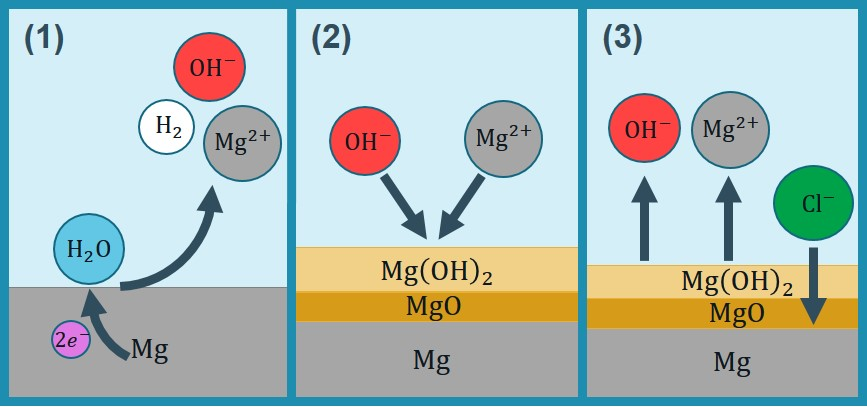
\includegraphics[width=10cm]{chemistry}
\caption{The chemistry of biodegradation of Mg considered in the current study: 1) Mg oxidation and water reduction processes accompanied by releasing $\mathrm{Mg}^{2+}$ and $\mathrm{OH}^{-}$  ions as well as $\mathrm{H}_2$ gas, 2) formation of a partially protective precipitation layer, 3) dynamic solubility equilibrium and contribution of $\mathrm{Cl}^{-}$.} \label{fig:chemistry}
\end{figure}

\subsection{Mathematical modeling}

To keep track of the concentration changes of various contributing chemical components, we define four state variables for the concentration of $\mathrm{Mg}^{2+}$ ions, protective film ($\mathrm{Mg}(\mathrm{OH})_{2}$), chloride ($\mathrm{Cl}^{-}$) ions, and the hydroxide ($\mathrm{OH}^{-}$) ions:
\begin{equation} \label{eq:state_vars}
\begin{aligned}
&C_{\mathrm{Mg}} = C_{\mathrm{Mg}}(\mathbf{x},t), \quad C_{\mathrm{Film}} = C_{\mathrm{Film}}(\mathbf{x},t)  \\
&C_{\mathrm{Cl}} = C_{\mathrm{Cl}}(\mathbf{x},t), \quad C_{\mathrm{OH}} = C_{\mathrm{OH}}(\mathbf{x},t) \quad \mathbf{x} \in \Omega \subset \mathbb{R}^{3}
\end{aligned},
\end{equation}
which are indeed 4 scalar functions of space and time. $\Omega$ denotes the whole region of interest, including both the Mg bulk and its surrounding medium. By doing this, the value of pH at each point of $\Omega$ can be calculated as:
\begin{equation} \label{eq:ph}
\mathrm{pH} = 14 + \log_{10}{C_{\mathrm{OH}}},
\end{equation}
where $C_{\mathrm{OH}}$ implies the activity of $\mathrm{OH}^{-}$. By having the definition of the state variables in Eq. \ref{eq:state_vars}, the biodegradation of Mg described by Eqs. \ref{eq:oxidation_react} and \ref{eq:break_react} can be represented as a set of reaction-diffusion PDEs:
\begin{equation} \label{eq:pde_mg}
\frac{\partial C_{\mathrm{Mg}}}{\partial t}=\nabla \cdot \left(D_{\mathrm{Mg}}^{e}  \nabla C_{\mathrm{Mg}} \right)-k_{1} C_{\mathrm{Mg}}\left(1-\beta \frac{C_{\mathrm{Film}}}{[\mathrm{Film}]_{\max }}\right) +k_{2} C_{\mathrm{Film}} {C_{\mathrm{Cl}}}^{2}
\end{equation}
\begin{equation} \label{eq:pde_film}
\frac{\partial C_\mathrm{Film}}{\partial t}=k_{1} C_{\mathrm{Mg}}\left(1-\beta \frac{C_{\mathrm{Film}}}{[\mathrm{Film}]_{\max }}\right) -k_{2} C_{\mathrm{Film}} {C_{\mathrm{Cl}}}^{2}
\end{equation}
\begin{equation} \label{eq:pde_cl}
\frac{\partial C_{\mathrm{Cl}}}{\partial t}=\nabla \cdot \left(D_{\mathrm{Cl}}^{e}  \nabla C_{\mathrm{Cl}} \right)
\end{equation}
\begin{equation} \label{eq:pde_oh}
\frac{\partial C_{\mathrm{OH}}}{\partial t}=\nabla \cdot \left(D_{\mathrm{OH}}^{e}  \nabla C_{\mathrm{OH}} \right)+k_{2} C_{\mathrm{Film}} {C_{\mathrm{Cl}}}^{2}
\end{equation}
in which the maximum concentration of the protective film can be calculated according to its porosity ($\epsilon$) \cite{Bajger2016}:
\begin{equation} \label{eq:film_max}
[\mathrm{Film}]_{\max }=\rho_{\mathrm{Mg}(\mathrm{OH})_{2}} \times(1-\epsilon).
\end{equation}
$D^e$ is the effective diffusion coefficient for each component. Due to the formation of the protective film, the diffusion coefficient is not constant and varies from the actual diffusion coefficient of the ions to a certain fraction of it. This fraction can be defined as ${\epsilon}/{\tau}$ \cite{Grathwohl1998,Hoeche2014}, in which $\epsilon$ and $\tau$ are the porosity and tortuosity of the protective film, respectively. The effective diffusion coefficient can be then calculated by interpolating the two aforementioned values:
\begin{equation} \label{eq:diff_coeff}
D_{i}^{e}=D_{i}\left(\left(1-\beta \frac{C_{\mathrm{Film}}}{[\mathrm{Film}]_{\max }}\right)+\beta \frac{C_{\mathrm{Film}}}{[\mathrm{Film}]_{\max }} \frac{\epsilon}{\tau}\right).
\end{equation}
The $\beta$ coefficient is called momentum here and controls the effect of the saturation term $(1-\frac{C_{\mathrm{Film}}}{[\mathrm{Film}]_{\max }})$. 

\subsection{Capturing the moving corrosion interface}

In \biodeg{}, the corrosion front is tracked using an implicit function such that the zero iso-contour of the function represents the metal-solution interface. As a common practice, this implicit function is expressed as a signed distance function that defines the distance of each point of space (the domain of interest) to the interface. Such a definition implies that the zero iso-contour of the function belongs to the interface. The level set method provides an equation to declare such an implicit function, $\phi=\phi(\mathbf{x},t), \mathbf{x} \in \Omega \subset \mathbb{R}^{3}$, which can be obtained by solving \cite{RonaldFedkiw2002}:
\begin{equation} \label{eq:lsm_full}
\frac{\partial \phi}{\partial t}+{\overrightarrow{V^\mathrm{E}} \cdot \nabla \phi}+{\mathrm{V}^\mathrm{N}|\nabla \phi|}={b \kappa|\nabla \phi|}
\end{equation}
in which $\overrightarrow{V^\mathrm{E}}$ is the external velocity field, and  $\mathrm{V}^\mathrm{N}$ is the value of the normal interface velocity. The last term is related to the curvature-dependent interface movement and is omitted. As the effect of perfusion is neglected in the current study, the term containing the external velocity is also eliminated, resulting in the following simplified form of the level set equation:
\begin{equation} \label{eq:lsm_simplified}
\frac{\partial \phi}{\partial t}+\mathrm{V}^\mathrm{N}|\nabla \phi|=0.
\end{equation}

By having the normal velocity of the interface ($\mathrm{V}^\mathrm{N}$) at each point and solving Eq. \ref{eq:lsm_simplified}, the interface can be captured at the zero iso-contour of the $\phi$ function.

In order to take advantage of the level set method for tracking the corrosion front, the velocity of the interface at each point should be determined. Then, by solving Eq. \ref{eq:lsm_simplified}, the interface is obtained at the points with a zero value of the $\phi$ function. The interface velocity in mass transfer problems can be calculated using the Rankine–Hugoniot equation \cite{Scheiner2007}, and by considering the transportation of $\mathrm{Mg}^{2+}$ ions, it can be written as:
\begin{equation} \label{eq:rankine}
\left\{\mathbf{J}(x, t)-\left([\mathrm{Mg}]_{\mathrm{sol}}-[\mathrm{Mg}]_{\mathrm{sat}}\right) \mathrm{V}(x, t)\right\} \cdot n=0
\end{equation}
where $\mathbf{J}$ is the mass flux at the interface. Rearranging Eq. \ref{eq:rankine} and inserting the value of the normal interface velocity into Eq. \ref{eq:lsm_simplified} yields:
\begin{equation} \label{eq:lsm_final}
\frac{\partial \phi}{\partial t}-\frac{D_{\mathrm{Mg}}^{e} \nabla_{n} C_\mathrm{Mg}}{[\mathrm{Mg}]_{\mathrm{sol}}-[\mathrm{Mg}]_{\mathrm{sat}}}|\nabla \phi|=0,
\end{equation}
which is the final form of the level set equation to be solved. 

\bibliographystyle{ieeetr}
\bibliography{refs}


\end{document}
